\documentclass[12pt,twoside]{article}
\usepackage[spanish,mexico]{babel}
\usepackage{natbib}
\usepackage{cite}
\usepackage{url}
\usepackage[utf8x]{inputenc}
\usepackage{amsmath}
\usepackage{mathtools}
\usepackage{graphicx}
\graphicspath{{images/}}
\usepackage{parskip}
\usepackage{fancyhdr}
\usepackage{vmargin}
\usepackage{hyperref}
\usepackage{xcolor}
\usepackage{braket}
\usepackage{float}
\setmarginsrb{3 cm}{2.5 cm}{3 cm}{2.5 cm}{1 cm}{1.5 cm}{1 cm}{1.5 cm}

\title{Sistema de imagen de absorción para la caracterización de una MOT.}								% Title
\author{Diego Martínez Cara}								% Author
\date{\today}											% Date

\makeatletter
\let\thetitle\@title
\let\theauthor\@author
\let\thedate\@date
\makeatother

\pagestyle{fancy}



\hypersetup{
    colorlinks = true,
    linkbordercolor = white,
	linkcolor = black,
	citecolor = blue,
	urlcolor = red,}
	
\begin{document}


\thispagestyle{empty}

\begin{minipage}[c][0.1\textheight][c]{0.2\textwidth}
\begin{center}
    
\includegraphics[width=3.3cm, height=3.3cm]{unam.png}
\end{center}
\end{minipage}
\begin{minipage}[c][0.1\textheight][t]{0.85\textwidth}
\begin{center}
    {\scshape Universidad Nacional Aut\'onoma de M\'exico}
    \vspace{.3cm}
    \hrule height2.5pt
    \vspace{.1cm}
    \hrule height1pt
    \vspace{.3cm}
    {\scshape  Facultad de Ciencias}
\end{center}
\end{minipage}

\begin{minipage}[c][0.8\textheight][t]{0.2\textwidth}
\begin{center}
\vspace{0.1cm}
\hskip2pt
\vrule width2.5pt height15cm
        \hskip1mm
        \vrule width1pt height15cm \\
        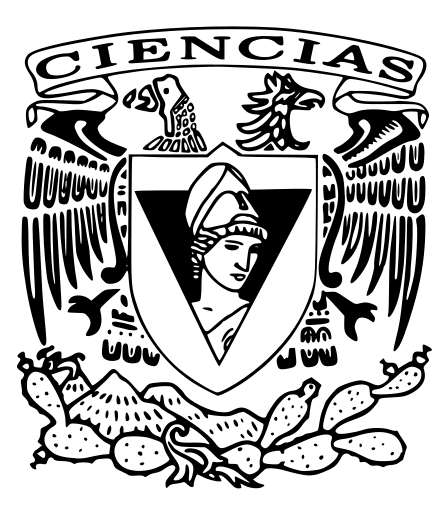
\includegraphics[height=3cm]{LogoCiencias.png}
        \end{center}
\end{minipage}
\begin{minipage}[c][0.6\textheight][t]{0.85\textwidth}
  \begin{center}
    {\Large \scshape {Sistema de imagen de absorción para la caracterización de una trampa magneto-óptica.}}

    \vspace{2cm}


    \makebox[5.5cm][c]{\LARGE TESIS}  \\[8pt] \vspace{2cm}
    QUE PARA OBTENER EL T\'ITULO DE:\\[5pt]
    {\large \textbf{{FÍSICO}}}\\[40pt]            
    PRESENTA:\\[5pt]
    \textbf{{DIEGO MARTÍNEZ CARA}}

    \vspace{1cm}

    {\small DIRECTOR DEL TRABAJO:\\ {DR. DANIEL SAHAGÚN SÁNCHEZ}}

    \vspace{0.5cm}

    {Ciudad Universitaria, Cd. Mx.,}{ }{2018}
  \end{center}
\end{minipage}

\clearpage
\begin{center}
\Large \textbf{Hoja de Datos del Jurado}
\end{center}
\small

1.Datos del alumno\\
Martínez\\
Cara\\
Diego\\
55 2092 2003\\
Universidad Nacional Autónoma de México\\
Facultad de Ciencias \\
Física\\
413012902
\vspace{0.2cm}\\
2. Datos del tutor\\
Dr\\
Daniel\\
Sahagún\\
Sánchez
\vspace{0.2cm}\\
3. Datos del sinodal 1\\
Dra\\
\\
\\
\vspace{0.2cm}\\
4. Datos del sinodal 2 \\
Dra\\
\\
\\
\vspace{0.2cm}\\
5. Datos del sinodal 3 \\ 
Dr\\
\\
\\
\vspace{0.2cm}\\
6. Datos del sinodal 4 \\
Dr\\
\\
\\
\vspace{0.2cm}\\
7.Datos del trabajo escrito\\
Desigualdades de Bell\\
Un experimento sencillo para la licenciatura\\
37 p\\
2016


\clearpage

\section*{}

\vspace{2cm}
\normalsize

\begin{flushright}
\textit{A José Cara Charda,}\\
\textit{uno de aquellos.}
\end{flushright}

\clearpage

\section*{Agradecimientos}

\clearpage

\section*{Resumen}



\clearpage

%%%%%%%%%%%%%%%%%%%%%%%%%%%%%%%%%%%%%%%%%%%%%%%%%%%%%%%%%%%%%%%%%%%%%%%%%%%%%%%%%%%%%%%%%

\tableofcontents
% \pagebreak
\clearpage




%%%%%%%%%%%%%%%%%%%%%%%%%%%%%%%%%%%%%%%%%%%%%%%%%%%%%%%%%%%%%%%%%%%%%%%%%%%%%%%%%%%%%%%%%

\section{Introducción}\label{introduccion}

-Intro MOT \\
-FWM en MOT\\
-Trabajo en cuestion.\\


\section{Capítulo I: Theoretical Background}\label{problema}


\subsection{Trampa Magneto-Óptica}\label{MOT}

\subsection{Revisión Teórica (Jen)}\label{JENteorev}

\subsection{Sístema de Imagen}\label{absorción}

Para recabar información sobre la nube de átomos se utiliza un sistema de imagen. En nuestro caso se utilizan dos técnicas, fluorescencia y absorción. 
El primero consiste en recolectar parte de la luz dispersada por la nube. Esto resulta particularmente práctico en trampas magneto-ópticas como la nuestra ya que la nube está fluoresciendo constantemente siendo entonces razonablemente sencillo monitorearla con este método. La segunda técnica, que es en la que nos centraremos a lo largo de este trabajo, como su nombre lo indica se basa en la absorción de luz por parte de nuestro ensamble de átomos. Se utiliza un haz de imagen con una intensidad mucho menor a la intensidad de saturación de los átomos y se observa, con la ayuda de un CCD, la sombra que estos crean al absorber parte de la luz de dicho haz.\\
\begin{figure}[h]
    \begin{center}
        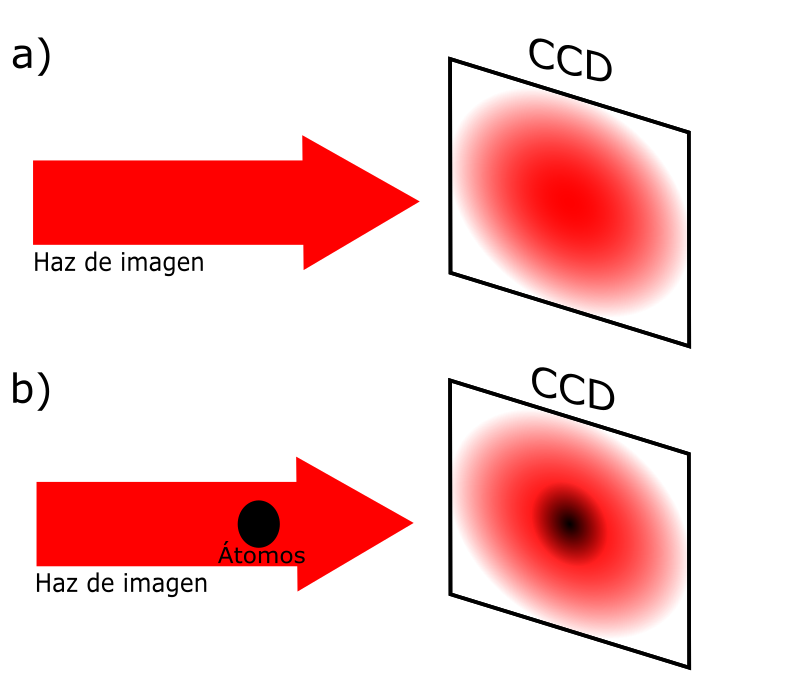
\includegraphics[width=0.6\linewidth]{esqabs.png}
    \end{center}
    \caption{Esquema de método de imagen por absorción: a)Imagen sin átomos. b)Imagen con átomos. }
    \label{esqimgabs}
\end{figure} \\
Este técnica presenta una mejor relación señal a ruido que la primera (la señal es al rededor de 100 veces mayor[citar Tesis de Gordon D. McDonald]) ya que con la primer técnica, debido a la distribución espacial isotrópica de la emisión de fotones en la fluorescencia, sólo capturamos parte de la luz dispersada. Sin embargo debemos tener en cuenta que el método de imagen por absorción no funciona para densidades ópticas demasiado grandes porque la transmisión decae exponencialmente con la densidad óptica causando que a densidades ópticas muy elevadas la sombra de la nube sea completamente obscura y no permita el un análisis adecuado. (De ser necesario, éste problema se puede solucionar desintonizando un poco el haz de imagen para sacarlo de resonancia.)\\ 
\subsubsection{Densidad óptica y número de átomos}\label{teoDOynum}

De acuerdo con la ley de Beer-Lambert, tras pasar por la nube de átomos el perfil de intensidades de la luz viene dado por:

\begin{equation}
%
    I_{T}(y,z) = I_{0}(y,z)T(y,z) = I_{0}(y,z) e^{-D(y,z)}.
%
\end{equation}

Aquí, la densidad óptica de la nube es:
\begin{equation}
%
    D(y,z) = \sigma_{\pi} n_{2D} = \sigma_{\pi} \int n_{0}(x,y,z) dx.
%
\end{equation}

Siendo $n_{2D}$ es la densidad de columna y $\sigma_{\pi}$ es el ángulo sólido de absorción que viene dado por:
\begin{equation}
%
    \sigma_{\pi} = \frac{\sigma_{0}}{1 + 4(\frac{\delta}{\Gamma})^2 + \frac{I}{I_{sat}}}.
%
\end{equation}

Notemos que para un haz cuya intensidad sea mucho menor que la intensidad de saturación de los átomos y que se encuentre en resonancia (o muy cerca de resonancia) tendremos que $\sigma_{\pi} \sim \sigma_{0}$ que en nuestro caso es igual a $1.938 \times 10^{-9} cm^2$.[citar el Steck]\\
\\
Por lo tanto, la señal que detectaremos al recolectar la luz después de la nube es:
\begin{equation}
    %
    F(y,z) = I_{T}(y,z) + B(y,z) = I_{0}(y,z)T(y,z) + B(y,z).
    %
\end{equation}
Donde $B(y,z)$ es el ruido de fondo que pueda percibir nuestro CCD.\\
\\
Para el límite de baja densidad óptica podemos entonces obtener la transmisión $T(y,z)$ y por lo tanto la densidad óptica $D(y,z)$ a partir de la señal detectada en nuestro CCD. Para lograrlo tomamos tres fotos. La primera $F_{1}(y,z)$, sin el haz ni la nube, nos va a dar las cuentas obscuras o ruido de fondo, es decir $F_{1}(y,z)=B(y,z)$. Luego tomamos una segunda foto $F_{2}(y,z)$, esta vez con el haz de imagen pero sin la nube de átomos obteniendo entonces $F_{2}(y,z) = I_{0}(y,z) + B(y,z)$ y finalmente tomamos la tercera imagen que nos da una señal como la descrita en la ecuación ().\\
\\
A partir de estas tres imágenes podemos calcular la densidad óptica de la nube: 
\begin{equation}
%
    D(y,z) = - ln\left(\frac{F(y,z)-F_{1}(y,z)}{F_{2}(y,z)-F_{1}(y,z)}\right).
%
\end{equation}

A partir de esto uno puede encontrar el número de átomos en la nube integrando sobre toda la imagen de la siguiente forma:
\begin{equation}
%
    N = \frac{A}{\sigma_\pi} \sum_{pixeles} -ln(T(y,z)).
%    
\end{equation}

Donde A es el área del píxel en el plano del objeto, es decir, $\frac{area del pixel}{magnificacion}$.

\subsubsection{Temperatura}\label{teotemp}


\section{Capítulo II: Experimento}\label{experimento}

\subsection{Operación de la MOT}\label{operacion}



\subsection{Sistema de imagen}\label{Sisimag}

\subsubsection{Sintonía fina de la frecuencia}\label{Sintonia}

En nuestro experimento nos interesa tener control sobre la frecuencia del haz de imagen para poder, por ejemplo, alejarlo de resonancia para hacer mediciones en nubes de mayor densidad óptica.\\
\\
Para conseguir este control sobre la frecuencia utilizamos Moduladores Acusto-Ópticos (AOM) de la marca IntraAction. Estos elementos están constituidos por un cristal dentro del cual se generan ondas de sonido gracias a las vibraciones de un transductor piezoeléctrico. Al propagarse dentro del material, estas ondas producen variaciones de presión y por lo tanto variaciones de índice de refracción que hacen que el sistema se comporte como una rejilla de difracción que podemos modular. Cuando un haz atraviesa el AOM se forma un patrón de difracción donde los diferentes ordenes presentan corrimientos de frecuencia. Dependiendo de la orientación relativa entre los vectores de onda del haz y de las ondas dentro del cristal el corrimiento será $\omega - \Omega $ (caso en el que las componentes correspondientes son paralelas) o $\omega + \Omega $ (caso en el que son anti-paralelas) en el orden con mayor intensidad.\\
\\
\begin{figure}[h]
    \begin{center}
        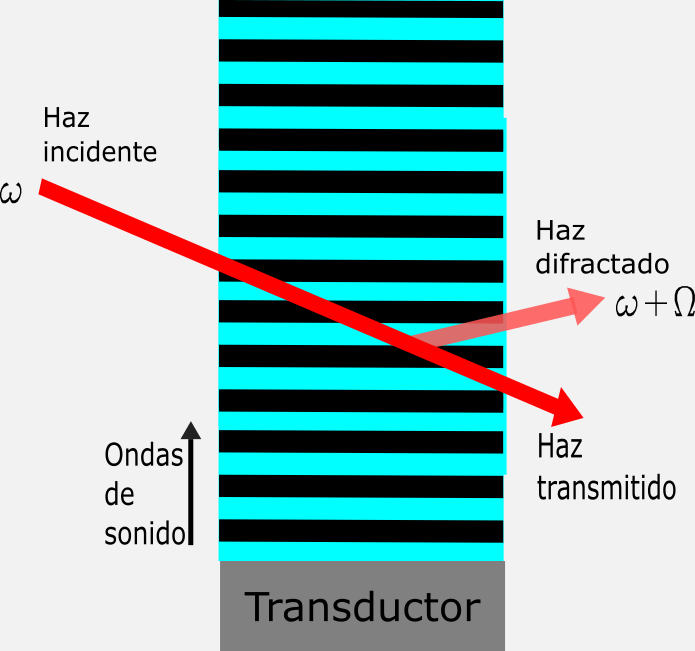
\includegraphics[width=0.6\linewidth]{Esquemaaom.png}
    \end{center}
    \caption{Esquema de un modulador acusto-óptico. }
    \label{esqaom}
\end{figure} \\
\newpage
Alineando cuidadosamente el orden que nos interesa y modulando con el controlador del AOM (marca *insertar marca*) tenemos control de hasta 0.001MHz sobre la frecuencia del haz. \\
\\
La luz utilizada para imagen proviene del láser maestro de nuestro laboratorio. Este láser está anclado al entrecruce $CO_{1-3}$ a alrededor de 211.8MHz de resonancia con la transición de enfriamiento $\ket{5S_{\frac{1}{2}},F=2} \rightarrow \ket{5P_{\frac{3}{2}},F'=3}$ del $^{87}Rb$. \\
Como se puede observar en la figura (\ref{arreglaom}), tomamos la luz para imagen de un PBS tras haber pasado por un primer AOM de +60MHz, es decir, que viene el haz a -151.8MHz de la transición de enfriamiento. De ahí lo mandamos en un doble paso a través de un segundo AOM, esta vez de +75MHz, recorriendo esta vez la frecuencia hasta -1.8MHz de la transición ya mencionada. El hacer esto en un doble paso, además de permitirnos reutilizar un mismo AOM para hacer dos corrimientos de frecuencia, nos permite evitar cambios de orientación en el haz al variar la frecuencia que podrían resultar en problemas con el acoplamiento de las fibras ópticas que distribuirán esta luz. [citar Donley, Double pass AOM system]\\
\\
Finalmente esta luz ya cerca de resonancia y cuya frecuencia ya podemos controlar se acopla a una fibra y en un arreglo posterior se divide pues será también utilizada para uno de los haces del FWM que se hará en etapas posteriores del experimento. 



\newpage
\begin{figure}[H]
    \begin{center}
        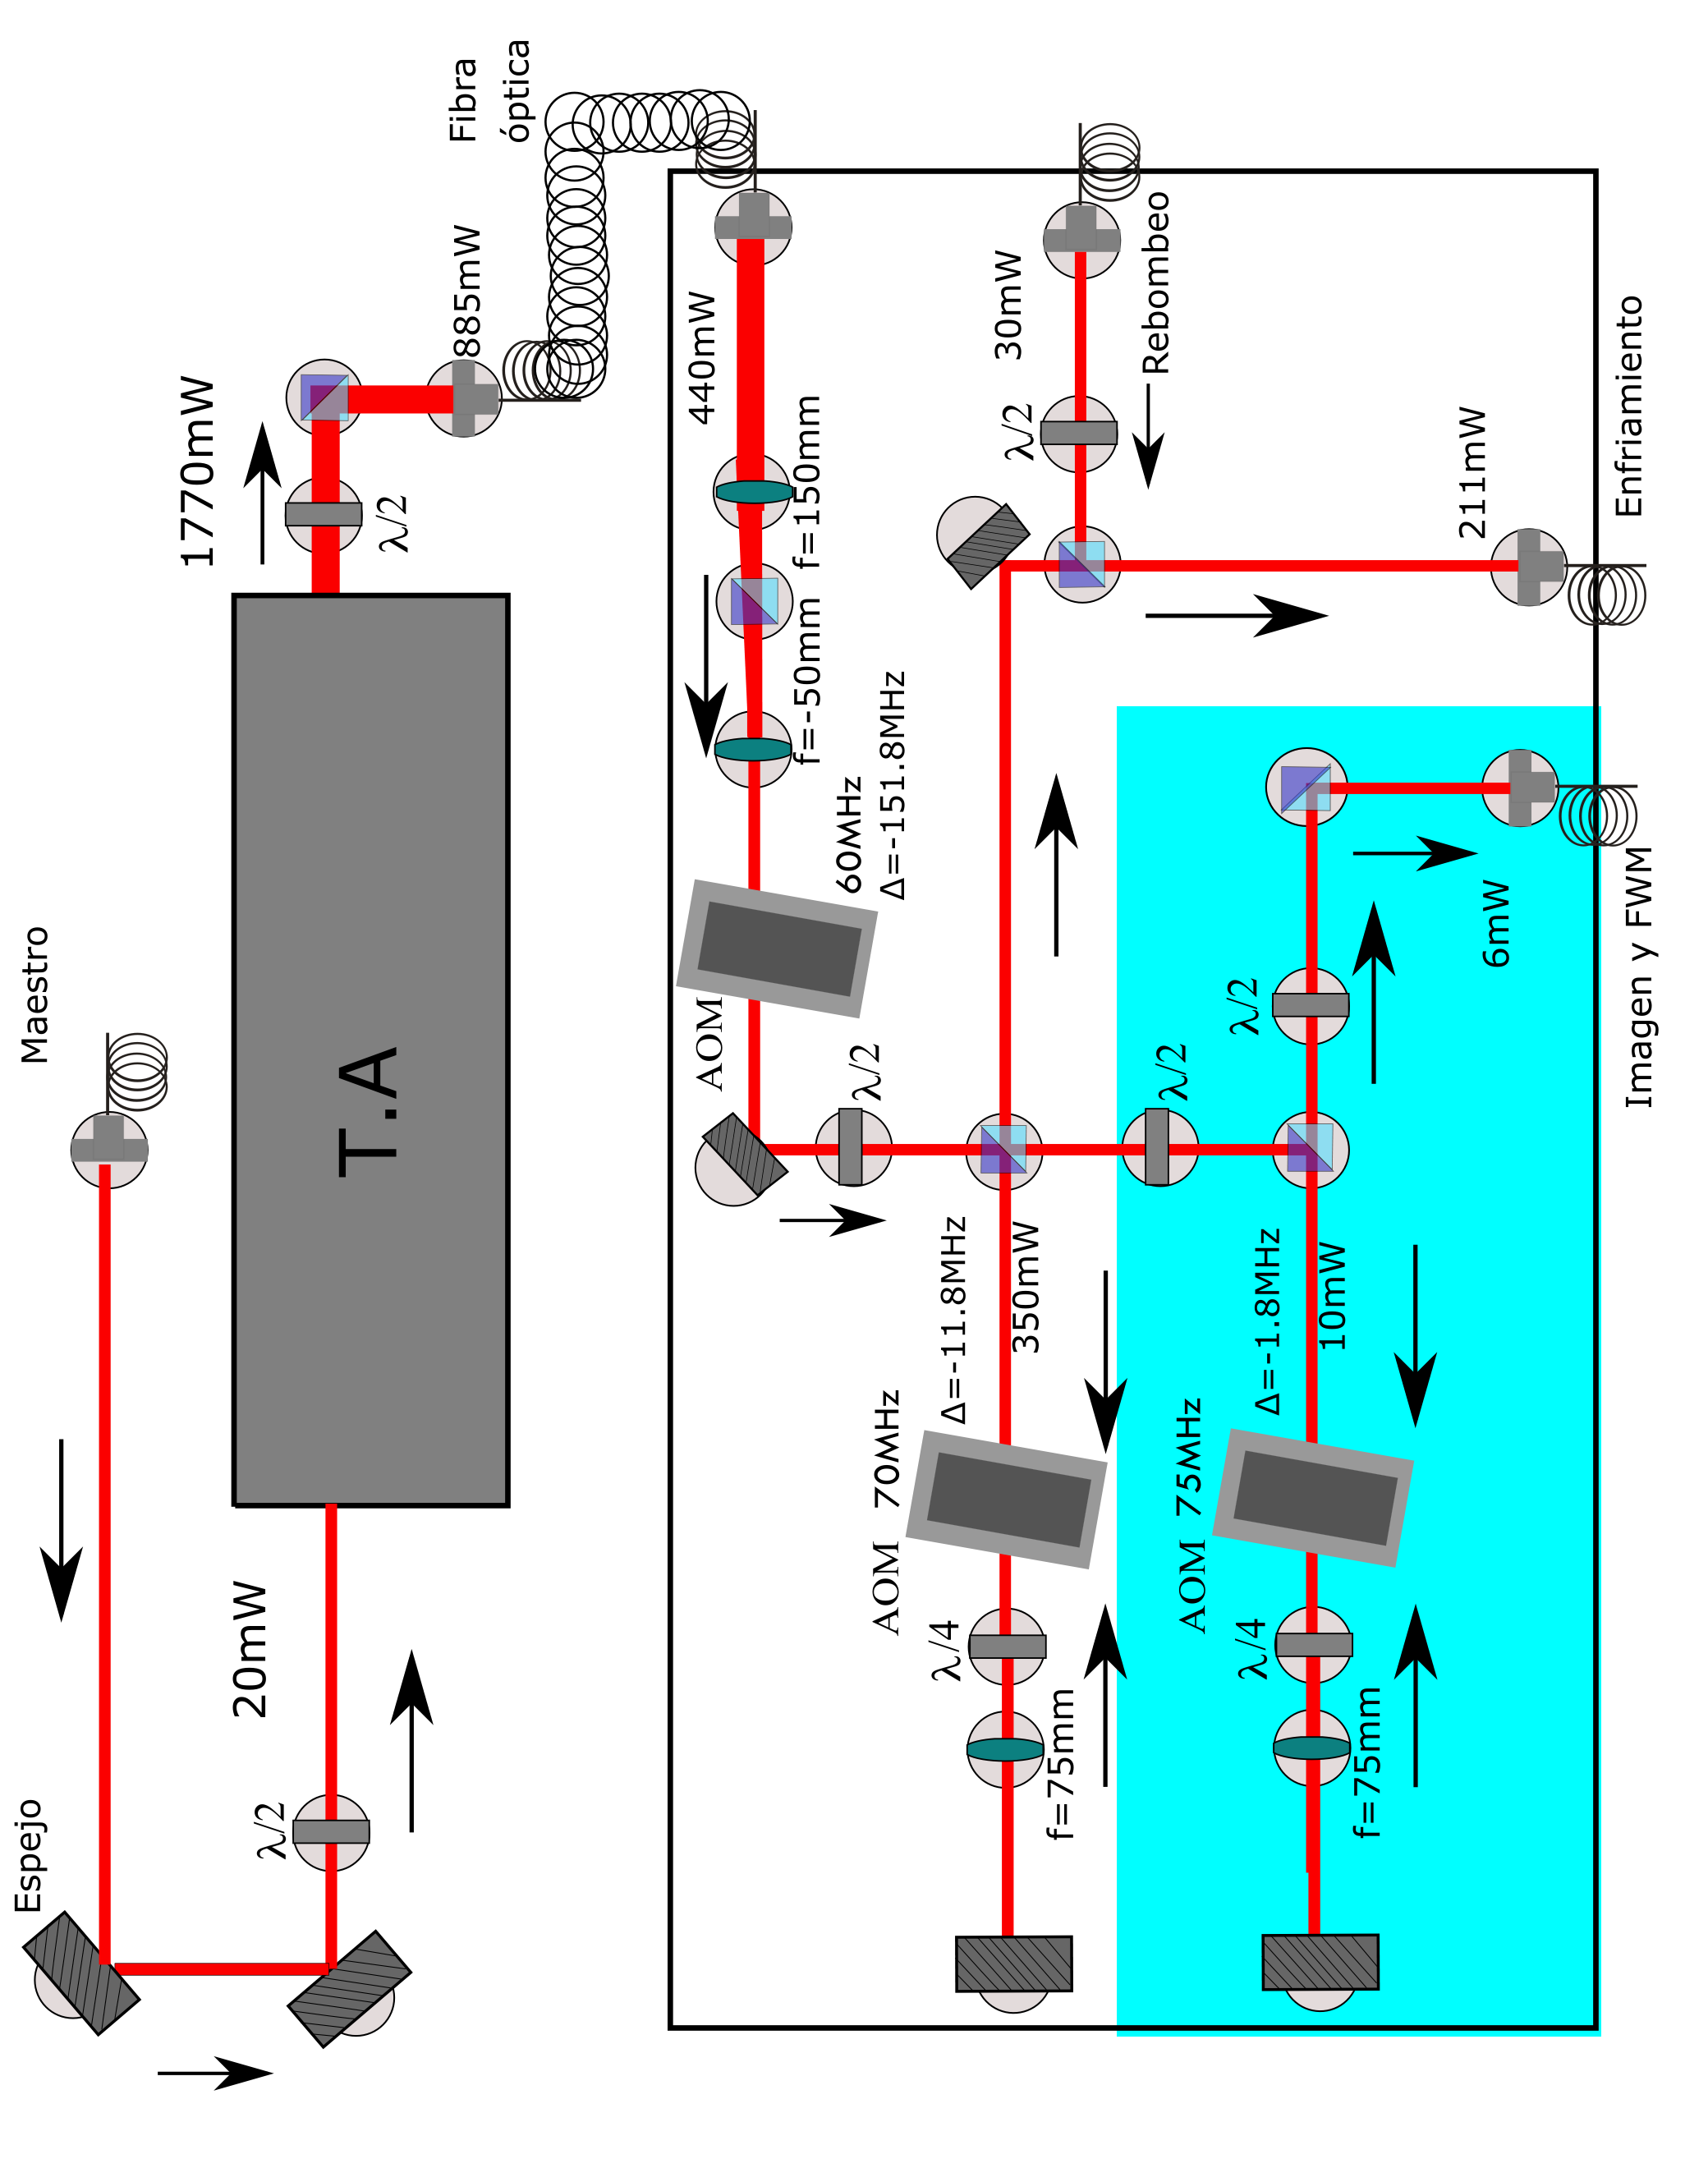
\includegraphics[width=1.1\linewidth]{amplificadoryAOM.png}
    \end{center}
    \caption{En la parte sombreada en azul celeste se muestra como, tras el primer AOM, parte de la luz pasa a una nueva parte del arreglo donde se realiza una segunda sintonía fina y su distribución para imagen y FWM.}
    \label{arreglaom}
\end{figure} 

\subsubsection{Arreglo de imagen}\label{Arreglo de imagen}

\subsubsection{Obturación}\label{obturacion}

\subsubsection{Adquisición}\label{manta}

\subsubsection{Control y sincronización}\label{control}


\section{Capítulo III: Resultados}\label{analisis}

\subsection{Optimización}\label{opt}

\subsubsection{Densidad Óptica}\label{do}

\subsubsection{Número de Átomos}\label{na}

\subsubsection{Temperatura}\label{tem}

\subsection{Control de regímenes de interés}\label{regimenes}



\section{Capítulo IV: Conclusiones}\label{Conclusiones}



\newpage
\bibliographystyle{myplain}
\bibliography{biblist}

\end{document}
